\section{МЕТОДЫ ИСПЫТАНИЙ}

\subsection{Испытание выполнения требований к программной документации}
     Состав программной документации проверяется визуально, проверяется наличие всех подписей и наличие программной документации в системе LMS. Также визуально проверяется соответствие документации требованиям ГОСТ.
     
     Документация действительно соответствует всем требованиям. Также дополнительно были проверены исходные тексты документов для проверки соответствия использования отступов и интервалов требованиям к выпускной квалификационной работе:
     
    \begin{figure}[H]
        \centering
        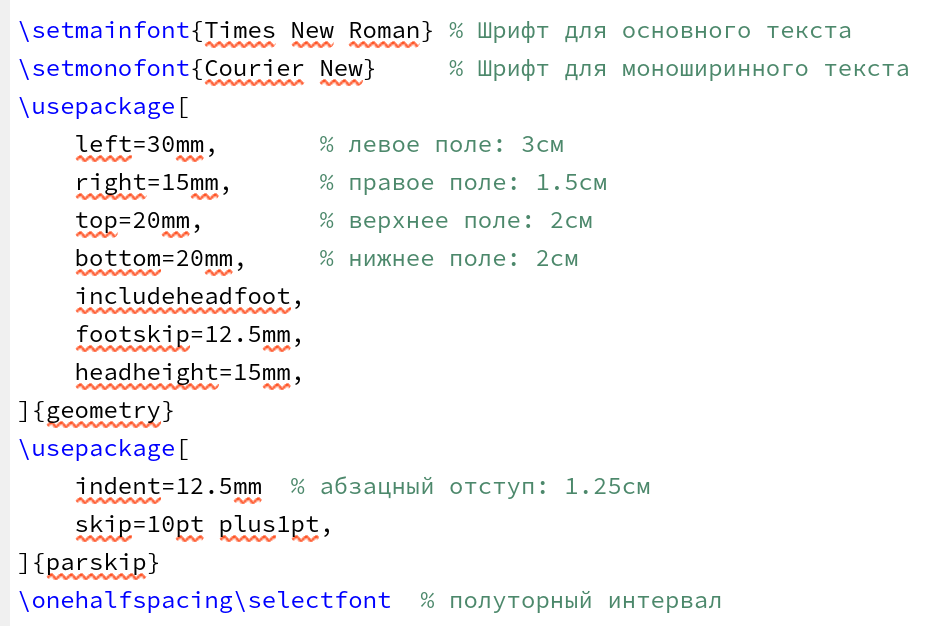
\includegraphics[width=0.5\textwidth]{figures/latex.png}
        \caption{Рекомендуемые параметры документов в системе LaTeX}
        \label{fig:my_label}
    \end{figure}

\subsection{Проверка требований к информационной и программной совместимости}
    Проверка осуществляется путем просмотра исходного кода программного проекта и прилагающейся к нему документации. В частности, проверяется использование системы контроля версий Git и что приложены все необходимые файлы для сборки проекта: исходные тексты, файлы Dockerfile.
    
    Это действительно так, в чем легко убедиться, благодаря просмотру файлов проекта на сайте GitHub.

\subsection{Проверка требований к функциональным характеристикам}
    Проверка осуществляется путем ручного тестирования сервиса с использованием исходных кодов самого сервиса в качестве входных данных.
    
    При тестировании необходимо сначала загрузить в систему результат индексации серверной части проекта, а также пользовательской части. Загрузка результатов индексации осуществляется в соответствии с руководством с использованием контейнера «shatterbird-indexer».
    
    Затем требуется вручную убедиться, что подсказки отображаются и работает функционал «перейти к определению» и «найти использования»: при использовании соответствующих кнопок действительно осуществляется переход в нужное место исходного кода.
    
    % \begin{figure}[H]
    %     \centering
    %     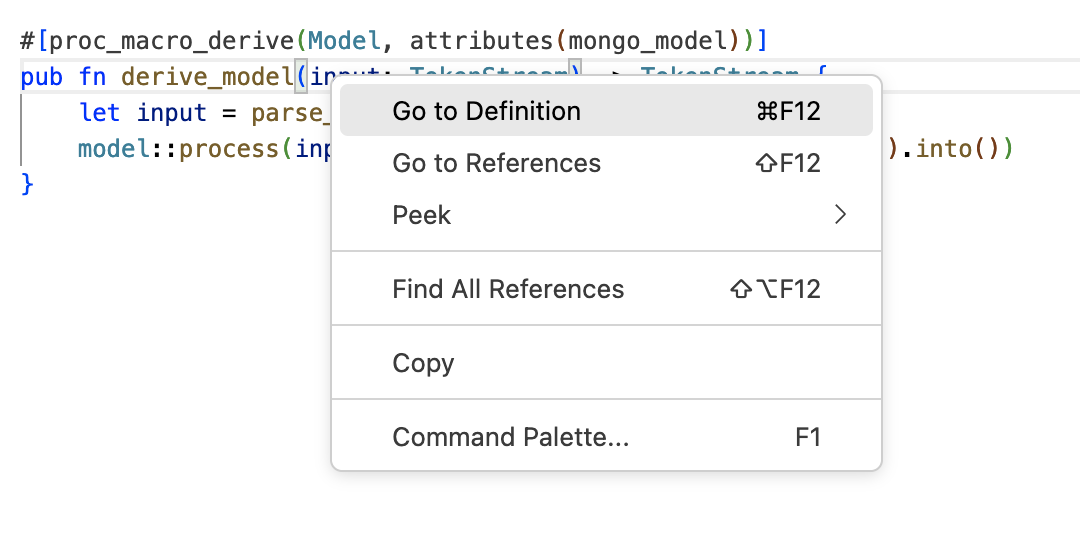
\includegraphics[width=0.5\textwidth]{figures/menu.png}
    %     \caption{Функционал «перейти к определению» и «найти использования»}
    %     \label{fig:my_label}
    % \end{figure}

\clearpage